\documentclass[uplatex,9pt]{jsarticle}
\usepackage{resume}
\usepackage{udline}
\usepackage{comment}
\usepackage[margin=0pt,font=small]{caption}
\usepackage{titlesec}
\usepackage{graphicx}
\usepackage{indentfirst}


\pagestyle{plain}

\titlespacing*{\section}{0pt}{6pt}{4pt}
\titlespacing*{\subsection}{0pt}{4pt}{2pt}

\setlength\intextsep{4pt}
\setlength\textfloatsep{4pt}
\setlength\floatsep{4pt}
\setlength{\parindent}{1zw}


\begin{document}

\twocolumn[
    \beginheader{2026年度 コンピュータサイエンス学部 中間発表}{2026}{8}{6}{井上 研究室}
    \title{VRにおけるブレス攻撃時の表示方法が視認性とゲーム体験に及ぼす影響}
    \author{C0B23049 北村 晴貴 (Haruki Kitamura)}
    \endheader
]

\vspace{3mm}
\setcounter{page}{1}


\section{はじめに}

ここ10年，VRゲームでは高い没入感を活かしたゲーム体験が求められている．
その中で，炎やビームなどの大規模な攻撃エフェクトは，戦闘の迫力や臨場感を高める重要な演出として広く利用されている．

しかし，大規模な攻撃エフェクトはプレイヤー自身の視界を遮る可能性があり，ターゲットの追従や照準操作が困難になることが考えられる．
その結果，視認性や操作性が低下し，ゲーム体験を損なう可能性がある．

一方で，攻撃エフェクトの透明化などによって遮蔽を軽減すると，迫力や没入感が低下する可能性がある．
そのため，視認性とゲーム体験を両立できる表示方法を明らかにすることが重要である．

そこで本研究では，VRにおけるブレス攻撃エフェクトに着目し，表示方法が視認性およびゲーム体験に与える影響を調査する．

\section{関連研究}

\begin{figure}[htbp]
\begin{center}
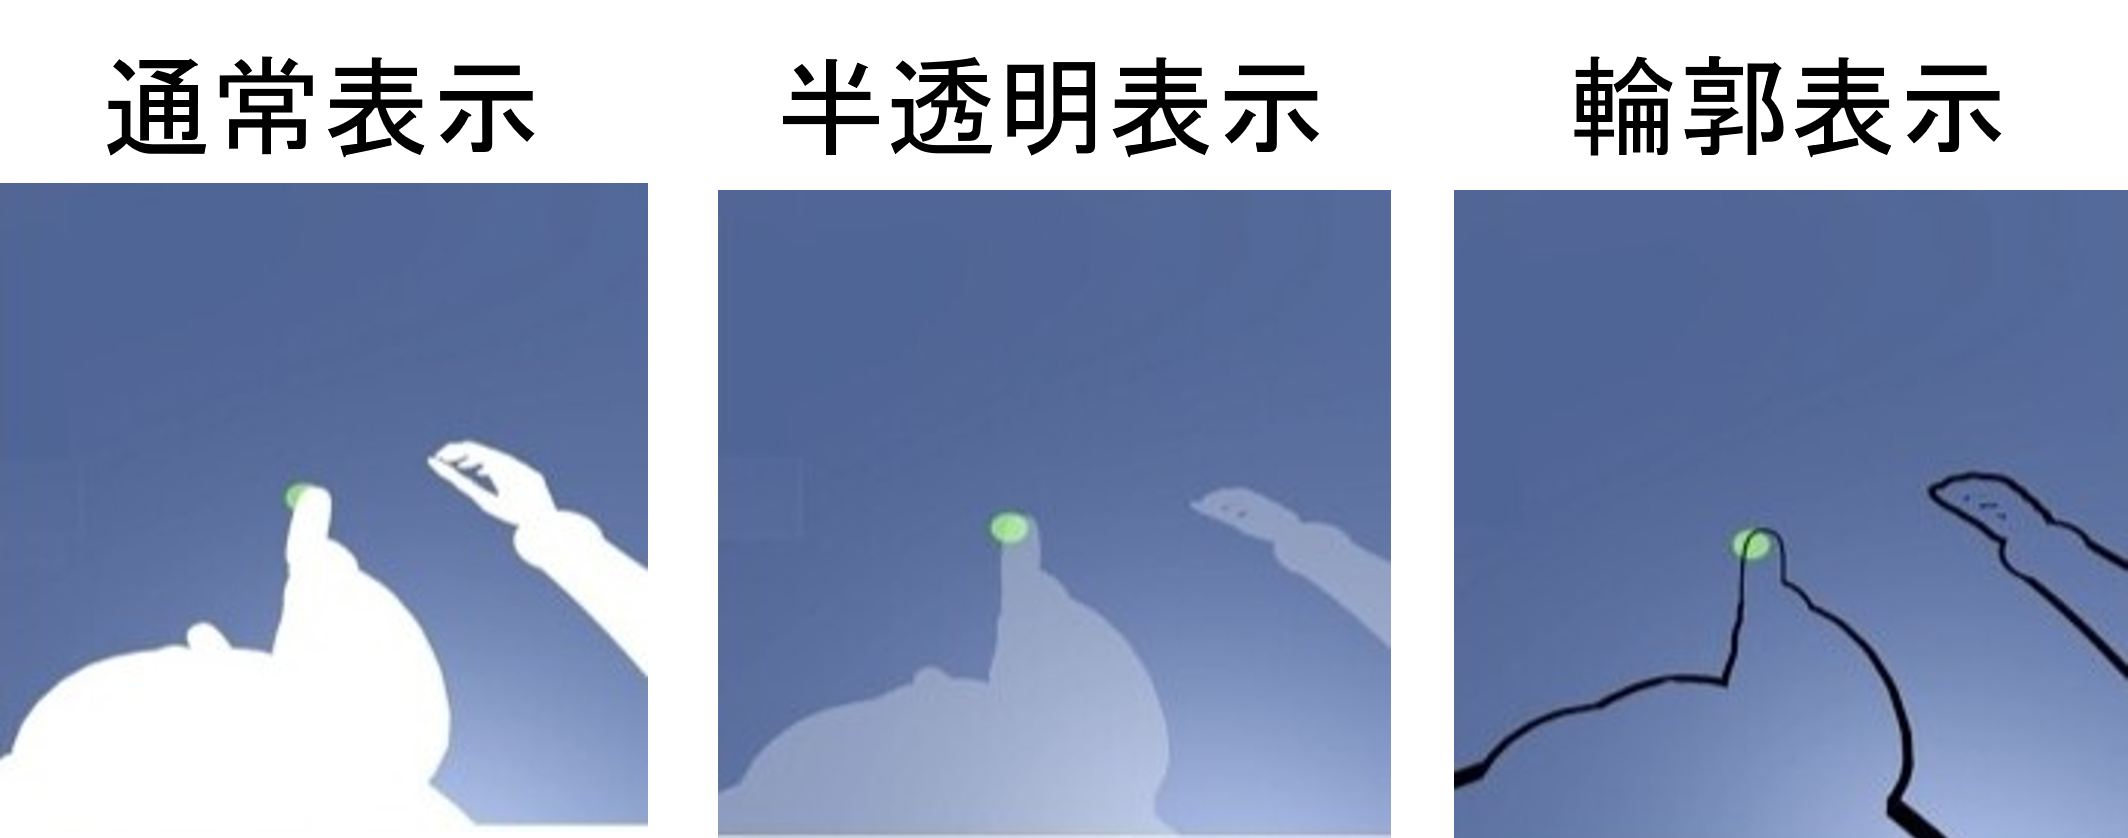
\includegraphics[width=0.85\linewidth]{fig/shih.png}
\caption{身体表示による遮蔽軽減手法}
\label{fig:shih}
\end{center}
\end{figure}


Shihらは，VR空間における身体による遮蔽を軽減するため，
身体表示方法を変更する手法であるSeeThroughBodyを提案した\cite{shih2025seethroughbody}．

実験では，通常表示，透明表示，輪郭表示など複数の身体表示条件を比較し，
表示方法によって視認性やタスク性能，ユーザ体験に影響を与えることを示した(\figref{fig:shih})．
しかし，この研究では身体による遮蔽を対象としており，
ユーザ自身が生成する攻撃エフェクトによる視界遮蔽については検討されていない．

そこで本研究では，攻撃エフェクトの表示方法に着目し，
視認性だけでなくゲーム体験への影響についても評価する．

\section{攻撃エフェクト表示手法} 

\subsection{システム概要} 本研究では，ブレス攻撃エフェクトによる視界遮蔽が視認性およびゲーム体験に与える影響を調査する．プレイヤーはブレス攻撃をランダム移動するターゲットに対して発射し，各表示条件を比較する． 


\subsection{ブレス攻撃エフェクト・ターゲットの表示方法}
ブレス攻撃エフェクトは対象物を遮蔽し，視認性を低下させる可能性がある．そこで本研究では，ブレス攻撃エフェクトとターゲットの表示方法を変更し，視界遮蔽の影響を軽減することを試みる．

以下の4種類の表示条件(\figref{fig:act7})を比較する．

\begin{itemize}
\item 通常表示
\item 半透明表示
\item 奥部透明表示
\item 輪郭表示
\end{itemize}

半透明表示では，エフェクト全体を透過することで対象物の視認性向上を図る．
奥部透明表示では，エフェクトの奥側のみを半透明にすることで，
攻撃の迫力を維持しながら対象物の遮蔽を軽減する．
輪郭表示では，エフェクトによって隠れた対象物の輪郭を表示することで，
対象物の位置を把握しやすくする．

これらの表示条件を比較し，視認性とゲーム体験への影響を評価する．

\begin{figure}[htbp]
\begin{center} 
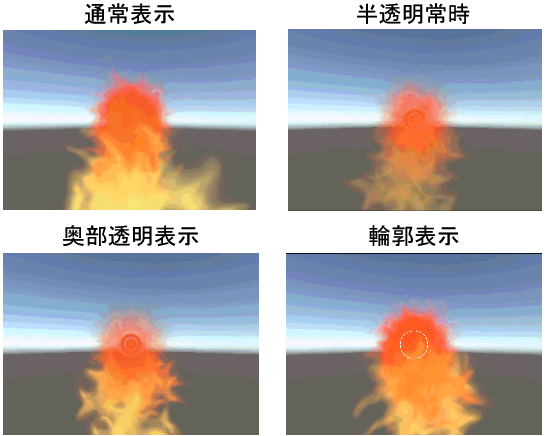
\includegraphics[width=0.85
\linewidth]{fig/fire.png} 
\caption{各表示条件の比較} 
\label{fig:act7}
\end{center}
\end{figure}

\section{実装}

本研究では，Unityを用いてブレス攻撃を行うVR環境を構築する．

攻撃エフェクトによる遮蔽の影響を比較するため，
通常表示，半透明表示，奥部透明表示，輪郭表示の4種類の表示方法を実装する．
また，評価実験で使用するターゲットを実装する．
ターゲットには，上下左右方向へランダム移動するものと，
放物線状にランダム移動し状態が変化するものを用いる．
状態変化を伴うターゲットでは，青色を攻撃可能状態，
赤色を攻撃不可状態として表示する．


\section{実験}

\subsection{ターゲット追従タスク}

表示方法による視認性への影響を評価するため，
ターゲット追従タスクを実施する．

被験者には，各表示条件において移動するターゲットへ30秒間ブレス攻撃を行ってもらう．
実験中はターゲット位置と照準位置を記録し，
両者の距離から追従性能を比較することで，各表示条件による視認性の違いを評価する．


\subsection{ターゲット攻撃タスク}

表示方法によるゲーム体験への影響を評価するため，
ターゲット攻撃タスクを実施する(\figref{fig:act3})．

被験者には，ランダムに移動する敵を攻撃し，
一分間でスコアを競ってもらう．
また，ブレス攻撃はチャージ制とし，
連続使用を制限することで，攻撃タイミングを考慮する環境を構築する．
さらに，攻撃不可状態の敵を攻撃した場合は減点することで，
敵の状態認識を必要とするゲーム環境を再現する．

\begin{figure}[htbp]
\begin{center} 
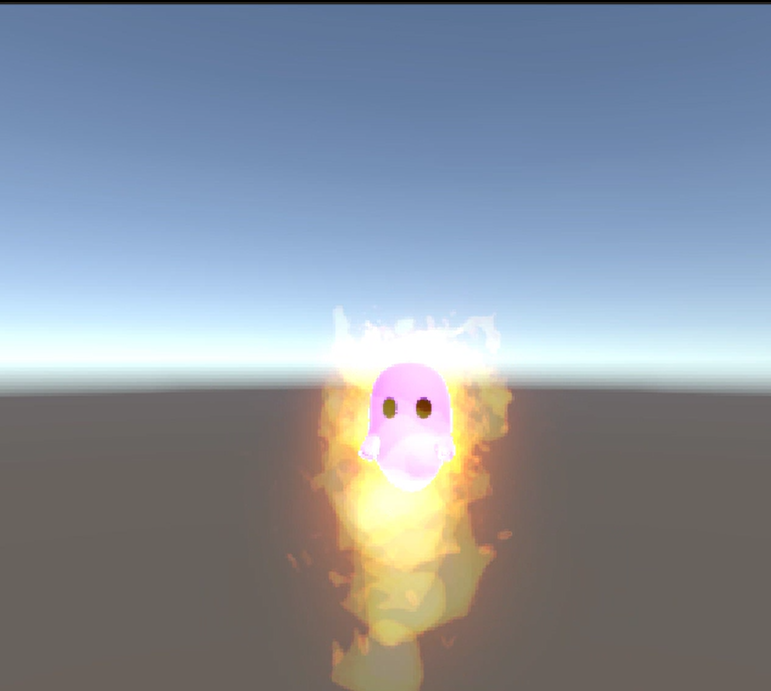
\includegraphics[width=0.65
\linewidth]{fig/exp1.png} 
\caption{ターゲットに攻撃中} 
\label{fig:act3}
\end{center}
\end{figure}

\section{評価方法}

\subsection{客観評価}

視認性の評価にはターゲット追従誤差を用いる(\figref{fig:act8})． 追従誤差はターゲット中心と照準中心との距離として定義し，値が小さいほどターゲットを正確に視認し，追従できていることを示す． 各表示条件における追従誤差を比較することで，表示方法が視認性に与える影響を評価する． 

\begin{figure}[htbp] 
\begin{center} 
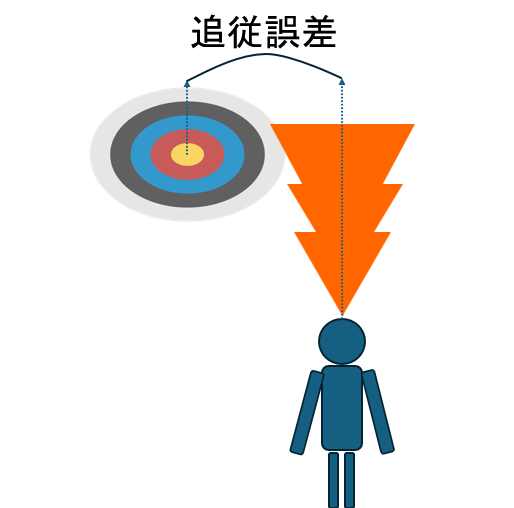
\includegraphics[width=0.68\linewidth]{fig/act8.png} 
\caption{追従誤差の説明} 
\label{fig:act8} 
\end{center} 
\end{figure}

\subsection{主観評価}

ターゲット攻撃タスク終了後にアンケートを実施する．

評価項目は視認性，没入感，迫力，満足度の4項目とし，
7段階評価によって各表示条件のゲーム体験への影響を比較する．

\begin{table}[htbp]
  \caption{主観評価アンケート項目}
  \label{tab:menu}
  \centering
  \begin{tabular}[h]{l|l}
    \hline
    \hline
    項目 & 質問項目 \\
    \hline
    Q1 & ターゲットの位置や動きが確認しやすいか \\
    Q2 & 自分がブレス攻撃を行っている感覚があったか \\
    Q3 & 攻撃エフェクトに迫力を感じたか \\
    Q4 & この表示方法でプレイしたいと思ったか \\
    \hline
  \end{tabular}
\end{table}

\section{まとめ}

本研究では，VRにおけるブレス攻撃エフェクトによる視界遮蔽に着目し，
視認性とゲーム体験を評価するためのシステムを提案した．
通常表示，半透明表示，奥部透明表示，輪郭表示の4種類の表示方法を実装し，
ターゲット追従タスクおよびターゲット攻撃タスクによって評価を行う．

今後は評価実験を実施し，各表示方法が視認性およびゲーム体験に与える影響を明らかにする．


\bibliographystyle{junsrt}
\bibliography{ref}

\end{document}